
%-----------------------------------------------------------------------------------
%-----------------------------------------------------------------------------------
%                                      PREAMBLE
%-----------------------------------------------------------------------------------
%-----------------------------------------------------------------------------------
\documentclass{article}
%-----------------------------------------------------------------------------------
% GENERIC PACKAGES
\usepackage[utf8]{inputenc}
\usepackage{amsmath}
\usepackage{graphicx}
\usepackage{hyperref}
\usepackage{setspace}
\usepackage[T1]{fontenc}
\usepackage{multicol}
\usepackage{caption}
\usepackage{textcomp}
\usepackage{blindtext}
\usepackage{tabularx}
\usepackage{layouts}
\usepackage{siunitx}
\usepackage{float}

\newenvironment{Figure}
  {\par\medskip\noindent\minipage{\linewidth}}
  {\endminipage\par\medskip}
%-----------------------------------------------------------------------------------
% GEOMETRY
\usepackage{geometry}
\geometry{
    left=25mm,
    right=25mm,
    top=25mm,
    bottom=25mm
    }
\onehalfspacing
\setlength\parindent{0pt}
%-----------------------------------------------------------------------------------
% ACRONYMS
\usepackage{acro}
\DeclareAcronym{hri}{
  short=HRI,
  long=Human-Robot Interaction,
}
\DeclareAcronym{mis}{
  short=MIS,
  long=minimally Invasive Surgery,
}
\DeclareAcronym{ramis}{
  short=RAMIS,
  long=Robot-Assisted Minimally Invasive Surgery,
}
\DeclareAcronym{vf}{
  short=VF,
  long=Virtual Fixture,
}
\DeclareAcronym{psm}{
  short=PSM,
  long=Patient-Side Manipulator,
}
\DeclareAcronym{mtm}{
  short=MTM,
  long=Master Tool Manipulator,
}
\DeclareAcronym{hrsv}{
  short=HRSV,
  long=High-Resolution Stereo Viewer,
}
\DeclareAcronym{ecm}{
  short=ECM,
  long=Endoscope Camera Manipulator,
}
\DeclareAcronym{ee}{
  short=EE,
  long=End-Effector,
}

%-----------------------------------------------------------------------------------
% NEW COMMANDS AND RENEW COMMANDS
\newcommand{\cright}{\textsuperscript{\textregistered}\phantom{..}}
\newcommand{\vect}[1]{\textbf{\textit{#1}}}
\newcommand{\fcaption}[1]{\captionof{figure}{\textit{\small #1}}}

\newcolumntype{A}{>{\centering\arraybackslash\hsize=1.1\hsize\linewidth=\hsize}X}
\newcolumntype{B}{>{\centering\arraybackslash\hsize=0.96666\hsize\linewidth=\hsize}X}
%-----------------------------------------------------------------------------------

% TITLE
\title{
\begin{figure}[h!]
\centering

\includegraphics[width=0.5\textwidth]{images/logo_polimi_scritta2.eps}
\end{figure}
\textbf{Implementation and assessment of Virtual Fixtures for VR Surgical Training with a \textit{daVinci} surgical robot: an experimental study}
\\
\vspace{0.5cm}\large{\textit{Politecnico di Milano - Master of Science in Biomedical Engineering}}
\\
\vspace{0.5cm}\textit{\small{Academic year 2022/2023}}\vspace{0.5cm}\\
{\large \textbf{Candidate: \textit{Alberto Rota}}\\
\textbf{Supervisor: \textit{prof. Elena De Momi}}\\
\textbf{Co-Supervisor: \textit{Ke Fan}}}}
\author{}
\date{}

%-----------------------------------------------------------------------------------
%-----------------------------------------------------------------------------------
%                                      BODY
%-----------------------------------------------------------------------------------
%-----------------------------------------------------------------------------------
\begin{document}
% TITLE
\maketitle
%-----------------------------------------------------------------------------------
% AUTHOR
% \vspace{1cm}
\begin{multicols}{2}
%-----------------------------------------------------------------------------------
\section{Introduction}
Since the introduction of \ac{ramis} in the healthcare market, patients have benefited from a diminishing of postoperative complications and an increase in the safety of procedures, while surgeons have been empowered by sophisticated robots which allowed the execution of complex tasks in adverse contexts. 
\newline
Surgical teams have been joined by robotic systems because of the number of benefits that result from the collaborative effort of the surgeon and the robot, combining the know-how and adaptation skills of the former and the high accuracy and stability of the latter. Such a synergistic perspective highlights the role of the \ac{hri} paradigm, which involves all aspects of understanding, designing, and evaluating robotic systems for use by or with humans \cite{Goodrich2007}. Most of the surgical robotics solutions on the market consist of a teleoperation console that interfaces with the practitioner and, separate from it, the surgical robot itself, which mimics the movements of the surgeon in real-time. This setup allows for higher motion accuracy, tremor filtration and magnified viewing of the surgical area; nonetheless tactile forces, friction and texture perception are excluded from the so crucial visuo-haptic feedback loop that would guide the surgeon in a standard ``non-robotic'' procedure.
\newline
This work, specifically, studies and evaluates the role of haptic Virtual Fixtures in the context of surgical training. \acp{vf} are high-level control strategies employed for assisting humans in man-machine collaboration tasks \cite{Bowyer2014}. In the context of surgical robotics, \acp{vf} assist the surgeon by providing haptic guidance at the level of the \textit{master} manipulator, generating mechanical forces and torques which re-direct the motion of the surgeon's hands. These assistance strategies may be most beneficial in the training process that aspiring surgeons undertake, which often takes place in a simulated virtual environment. Exploiting the customizability of simulated surgical tasks together with the implementation of \acp{vf} will enhance the process of learning key surgical skills, in terms of performance, retention and transfer.
\section{State of the art}
Surgical robotics companies usually commercialize a simulation framework in parallel to clinical robots. A survey of the most relevant training simulators on the market was conducted in \cite{Bric2016}: this review also assesses the suitability of virtual environments in comparison to that of dry-lab setups. However, since no commercially available clinical system implements a force-based assistive modality similar to that of virtual fixtures, none of the training simulators employ \acp{vf} either. The role of such assistive strategies in a real surgical scenario is still uncertain and shall be assessed only through an extensive clinical trial and, as a matter of fact, the vast majority of training protocols implementing \acp{vf} regards \textit{ad-hoc} systems like \cite{Lin2014}, which are limited both in terms of tasks implemented and in terms of evaluation protocols. Indeed, few studies \cite{Enayati2018} have evaluated the trainee's performance on multiple diverse tasks and over the course of multiple training days, and none has yet investigated the role of haptic assistance on skill retention and skill transfer. 

This work proposes an evaluation of the role of \acp{vf} in the context of surgical training with a multi-day experimental protocol articulated in two phases, designed in order to highlight the difference in the transfer and retention of skills between a control group and an assisted group. 
\section{Materials and methods}
\subsection{Surgical Simulator}
This research was conducted on a \textit{daVinci}\cright surgical robot integrated with the open-source dVRK \cite{Kazanzidesf2014} framework. The \acp{mtm} of the \textit{daVinci}\cright are in fact equipped with motors usually employed for the sake of homing and calibration; the \ac{vf} forces and torques are generated by energizing these motors according to the inverse kinematics of the manipulators. A ROS framework manages the communication between the teleoperation console of the dVRK and the virtual surgical scene, which is built upon the Unity\cright physics engine: therefore, the real \acp{psm} do not move during teleoperation, as the joint coordinates are communicated only to the virtual 3D objects.\newline
The simulator comprises eight surgical tasks, four of which (\textit{Path, Rings, Pillars} and \textit{Exchange}) are simplistic training tasks built with objects of simple geometry, while the remaining four (\textit{Liver Resection, Nephrectomy, Thymectomy} and \textit{Suturing}) emulate \textit{in-vivo} surgical procedures and are therefore more realistic. Fig.\ref{fig:taskspanel} collects snapshots of the tasks. All of these are constructed and set-up in order to be as challenging as possible in relation to a specific surgical skill. A set of fundamental pre-operative and intra-operative skills that any robotic surgeon should acquire during training was proposed in \cite{Smith2014}. Specifically:
\begin{figure*}
  \centering
      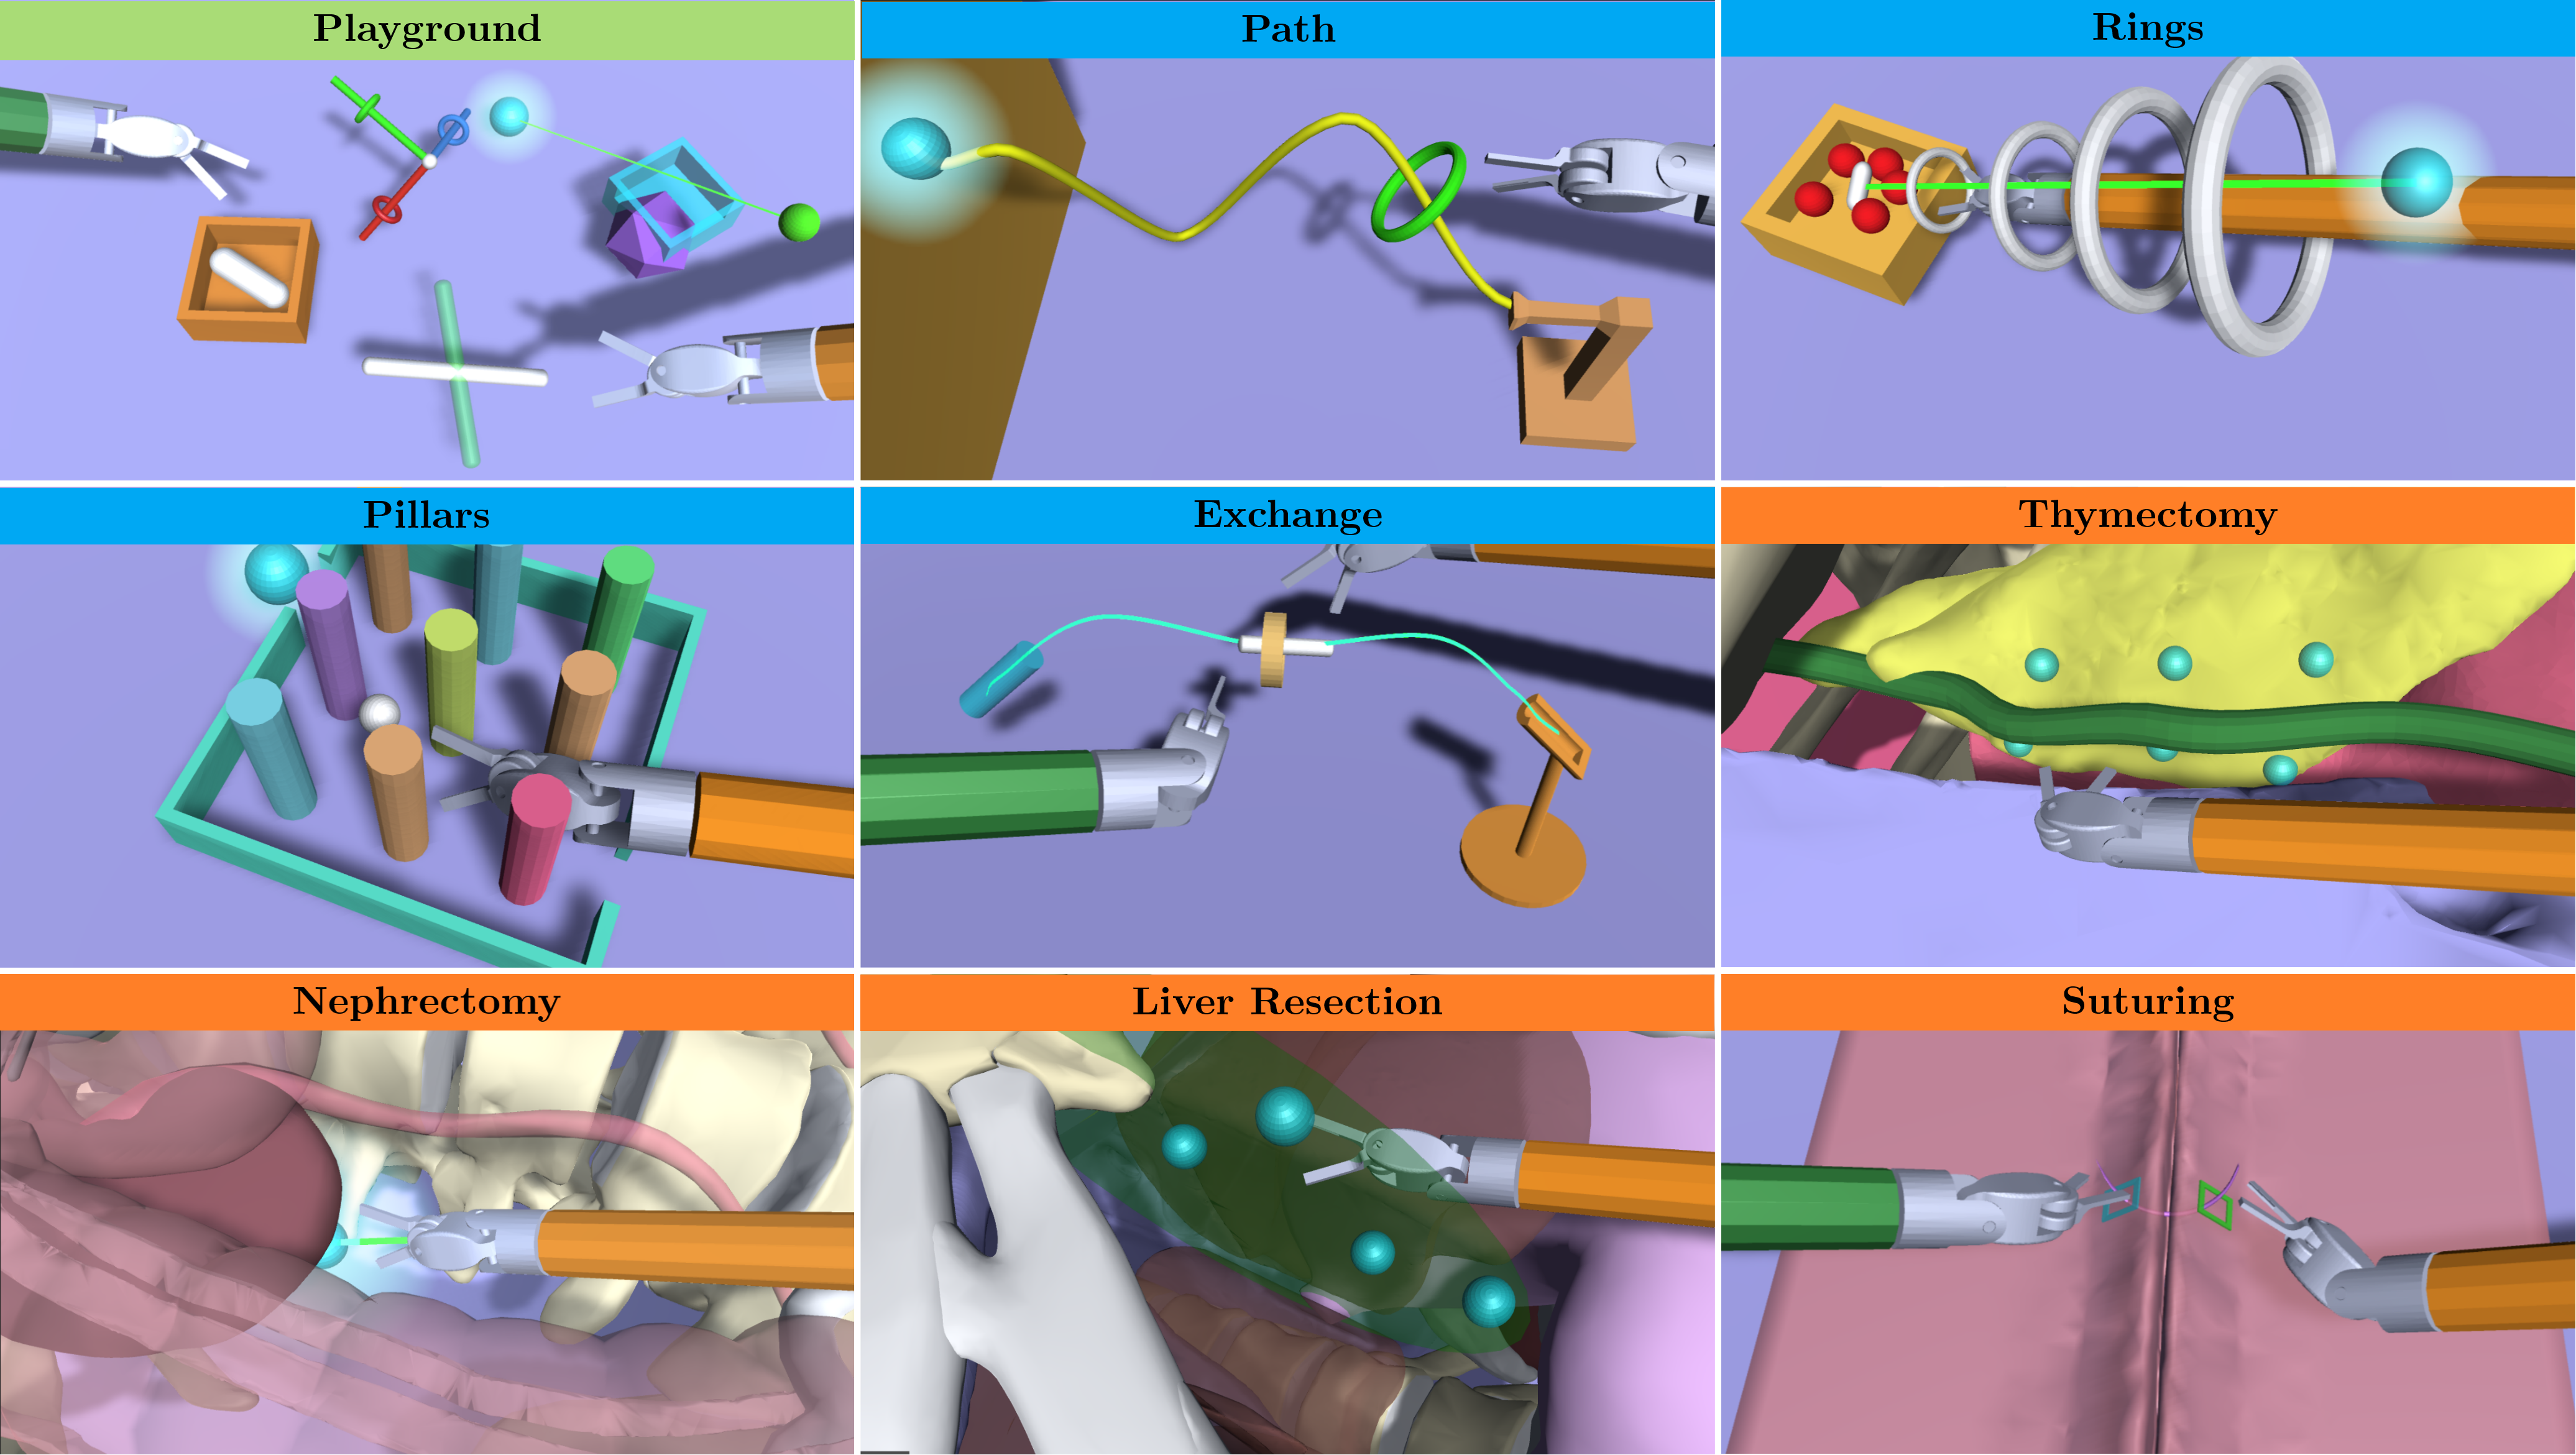
\includegraphics[width=\linewidth]{images/PANEL_named.png}
      \caption{\small{\textit{Snapshot of the simulated surgical tasks, with the respective denomination. Training tasks have blue headlines, while realistic evaluation tasks have orange headlines. \textit{Playground} is a propaedeutic task and isn't featured in the}}}
      \label{fig:taskspanel}
\end{figure*}
\begin{itemize}
  \item \textit{Path} and \textit{Liver Resection} require articulate wrist motion and stability
  \item \textit{Rings} and \textit{Nephrectomy} survey the depth perception skills
  \item \textit{Pillars} and \textit{Thymectomy} are hand-eye coordination tasks
  \item \textit{Exchange} and \textit{Suturing}, both bi-manual tasks, challenge the capabilities in terms of instrument exchange 
\end{itemize}
Since each training task has a corresponding emulated surgical procedure, the experimental phase will allow to evaluate the transferability of skills.
\newline
The simulator also exploits the 3D viewing capability of the \ac{hrsv} installed on the teleoperation surgical console: two virtual cameras are positioned in the Unity\cright scene at a distance of 5.3mm, with their feed being sent separately on the left and right oculars at the console achieving a three-dimensional perception of the virtual environment.
\subsection{Virtual Fixtures}
During teleoperation the surgeon is de-coupled from the patient: this is necessary in order to exploit the benefits of a robotic solution, which requires the system to be ``in between'' the practitioner and the patient in order to enhance the surgical experience. However, this de-coupling removes the haptic component from the motion control feedback loop of the surgeon, who is used to relying on the sense of touch when operating with a conventional approach. For this reason, this work analyses how the introduction of haptics in a virtual surgical environment may enhance the training phase, acting as a guidance and error-correcting medium. \newline
In the context of Virtual Fixtures, also known as Active Constraints, a haptic force is applied to the manipulators at the surgical console, which re-directs the motion of the surgeon's hands in case of improper or unsafe maneuvers. The magnitude and direction of the \acp{vf} force are computed from the \ac{psm} position and orientation relative to the surgical space and the position of objects in the scene, in a true feedback fashion. A transformation matrix $T_{PSM}^{MTM}$ mapping the \ac{psm} operatory space to the \ac{mtm} console space is necessary in order to sensibly use the feedback force and torque as corrective media. 
\begin{equation}
  \vect{f}_{MTM} = T_{PSM}^{MTM}\cdot \vect{f}_{PSM}
  \label{eq:forcepsm2mtm}
\end{equation}
\begin{equation}
  \vect{t}_{MTM} = T_{PSM}^{MTM}\cdot \vect{t}_{PSM}
  \label{eq:torquepsm2mtm}
\end{equation}
Most of the assistance strategies implemented here will use the distance from the \ac{psm} to the target or obstacle as the primary metric for determining the intensity of the feedback force or torque. However, different surgical tasks and situations require a level of control over how the distance is taken into account, and for this reason a sigmoidal mapping function is employed for the normalization of the linear or angular error into a suitable interval. Specifically, such mapping is formulated as:
\begin{equation}
  f_{map}(x) = \frac{1}{1+e^{5\delta w(x-t-h)}}
  \label{eq:sigmoidalmap}
\end{equation}
with $\delta = +1$ for guidance \acp{vf} and $\delta = -1$ for avoidance \acp{vf}. Here:
\begin{itemize}
  \item $t$ is the fixture \textit{threshold}, hence the value at which the sigmoid starts to significantly increase from zero
  \item $h$ is the distance from the threshold at which \textit{half} of the maximum force is provided
  \item $w$ controls the \textit{width} of the linear region, hence the steepness of the curve 
\end{itemize}
For example, if $t=2\si{mm}$ and $h=3\si{mm}$ the surgeon will start to feel a force for errors higher than 2\si{mm}, and at 5\si{mm} he/she will experience half of the maximum force that can be delivered.
\begin{Figure}
  \centering
      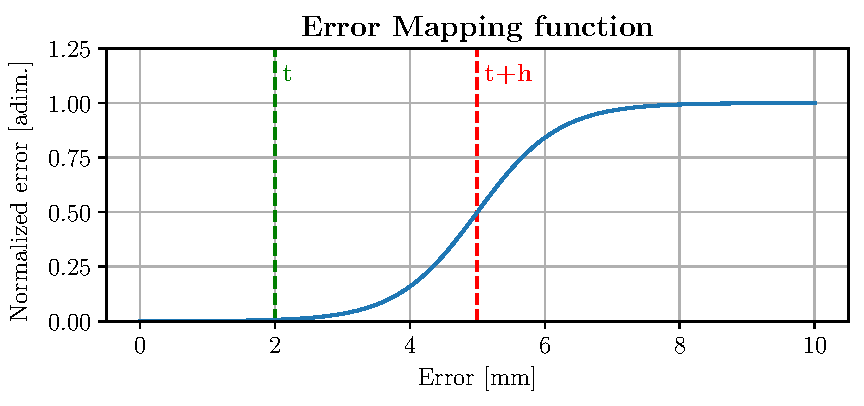
\includegraphics[width=\linewidth]{images/mappingfunction.eps}
      \fcaption{Plot of the Error Mapping function. The position of$t$ and $t+h$ can be set manually to achieve a suitable behavior of the assistance strategy\vspace{0.5cm}}
      \label{fig:mappingfunctiion}
\end{Figure}
For the purpose of stability and, therefore, safety in the assistive feedback loop, all the \acp{vf} implemented have an elastic component, proportional to the error mapped with the sigmoidal function, and a viscous component proportional to its rate of change, which damps the possible oscillatory instabilities. The optimal visco-elastic balance is heavily task-dependent and surgeon-dependent, and for this reason it is tuned by manually setting the values of $K_f$, $K_T$, $\eta_f$ and $\eta_T$ in the equations
\begin{equation}
  \vect{f} = K_f\cdot\vect{f}_{elastic} + \eta_f\cdot\vect{f}_{viscous} 
  \label{eq:forcevfbalance}
\end{equation}
\begin{equation}
  \vect{t} = K_t\cdot\vect{t}_{elastic} + \eta_t\cdot\vect{t}_{viscous} 
  \label{eq:torquevfbalance}
\end{equation}    
which will ultimately result in the haptic outputs provided to the actuators.
\newline
The four types of \acp{vf} featured in the surgical simulator are described in the following paragraphs:
\paragraph{Trajectory Guidance} Given a reference trajectory - planned in the pre-operative phase - this \ac{vf} steers the surgeon's hands in order to align the robotic \ac{ee} with the closest point on the trajectory itself. The feedback force attracts the \ac{ee} towards the reference, while the torque rotates it so that it's aligned with the tangent vector at the closest point. 
\paragraph{Insertion Guidance} This \ac{vf} aids the surgical insertion of the \ac{ee} towards a target point, maintaining the path of the tooltip stable inside an insertion cone. Here the feedback force has the same direction as the radial conical coordinate and a magnitude that is proportional both to the distance to the cone centerline and the distance to the target point. With this configuration, the \ac{psm}'s tooltip will be kept inside the reference insertion cone.
\paragraph{Surface Guidance} Similarly to the \textit{Trajectory Guidance} \ac{vf}, the distance vector to the closest point belonging to a reference surface (planar or non-planar) determines the force feedback, while the torque aligns the \ac{ee} to the tangent plane at the closest point.
\paragraph{Obstacle Avoidance} Having identified a 3D mesh as an obstacle, the distance to the robotic tooltip and its rate of change are used for computing the force feedback. By setting $\delta = -1$ in Eq.\ref{eq:sigmoidalmap}, the sigmoidal mapping function is flipped and higher forces will be generated from small distance errors. 
\subsection{Clinical Validation}
Two resident surgeons from the \textit{Istituto Europeo di Oncologia}, both regularly performing \ac{ramis} procedures with the \textit{daVinci}\cright robot, kindly dedicated their time in testing the surgical simulator in all its aspects, from the motion truthfulness to the complexity of the wrist articulation to the invasiveness and visco-elastic balance of the virtual fixtures. Their opinion and expertise were precious and insightful tools that guided the development towards a clinically validated robotic surgical simulator. 
Moreover, the most expert resident surgeon allowed to have his performance recorded when practicing with the simulator, which will be considered ``peak performance'' in the experimental analysis. 
\subsection{Experimental Protocol}
The effectiveness of the haptic virtual fixture paradigm has been assessed with an experimental study where the performance of un-assisted subjects in a control group was compared to the one recorded from subject to whom was provided haptic assistance. Since the aim of this work is to establish the role of \acp{vf} in the training context, eight novice subjects with little to no experience with surgical robots were recruited for the study. Subjects were 25\% females and 75\% males, between 23 and 27 years of age, all right-handed and either had never teleoperated a surgical robot or did it less than 5 times. Assignation to the control or assisted group was random.
\newline
% !!!! CHANGE DAYS NUMBERING
The subjects underwent a week-long training phase:
\begin{itemize}
  \item On \textit{Day 1}, they were given a concise explanation about the \textit{daVinci}\cright surgical system, the simulator, haptics, and the training protocol. Later, each subject experienced 5 minutes in a \textit{Playground} environment (Fig.\ref{fig:taskspanel}), purposely designed to understand the elementary mechanics of teleoperation, clutching and object grasping. No performance metric was recorded at this time
  \item From \textit{Day 2} to \textit{Day 5} they were asked to execute the four training tasks of the simulator (\textit{Path, Rings, Pillars} and \textit{Exchange}), each one for a total of 3 repetitions. Tasks appeared sequentially in a random order, contributing to un-bias the results. At the beginning of each daily session, subjects could interact with the \textit{Playground} environment for 1 minute at maximum.
  \item On \textit{Day 6} and \textit{Day 7} subjects were given a break period and no training was performed
  \item On \textit{Day 8} they were asked to execute the four surgical evaluation tasks of the simulator (\textit{Thymectomy, Nephrectomy, Liver Resection} and \textit{Suturing}), each one for a total of 3 repetitions. Again, tasks appeared sequentially in a random order, contributing to un-bias the results.
\end{itemize}
\subsection{Metrics}
A quantitative estimation of surgical performance is obtained by combining metrics recorded in real time during the execution of the task. The simulator logs these metrics autonomously detecting when the user initiates the execution and when the task is completed, at a framerate of 30 Hz. The metrics are:
\begin{itemize}
  \item $D$: Distance error, from the \ac{ee} to the closest point of the target (trajectory, surface or object)
  \item $A$: Angular error, from the \ac{ee} to tangent vector in the closest point of the reference trajectory or to the tangent plane in the closest point of a surface
  \item $F$: Feedback force, computed from the \ac{vf}. The force is computed also for the subjects in the non-assisted control group, but it's not delivered during the operation
  \item $T$: Feedback torque, computed from the \ac{vf}. The torque is computed also for the subjects in the non-assisted control group, but it's not delivered during the operation
  \item $M$: Missed exchanges. When, in the bi-manual tasks, an object is dropped when passing it from the left \ac{psm} to the right, or vice versa
  \item $C$: Clutch time, the fraction of the total task time during which the clutch pedal was pressed for repositioning
\end{itemize} 
These values are logged at each frame of the task execution and are then averaged once the task is complete. These metrics are combined with a weighted average, the weights of which are dependent on the task and the key surgical skills that such a task requires. 
\newline
Considering ``optimal execution'' the one achieved by the resident surgeon, the quantitative performance index $P$ is the ratio of the task combined metrics gathered from the optimal execution from the surgeons and the one recorded from the training subjects. 
\section{Results}
\begin{figure*}
  \centering
      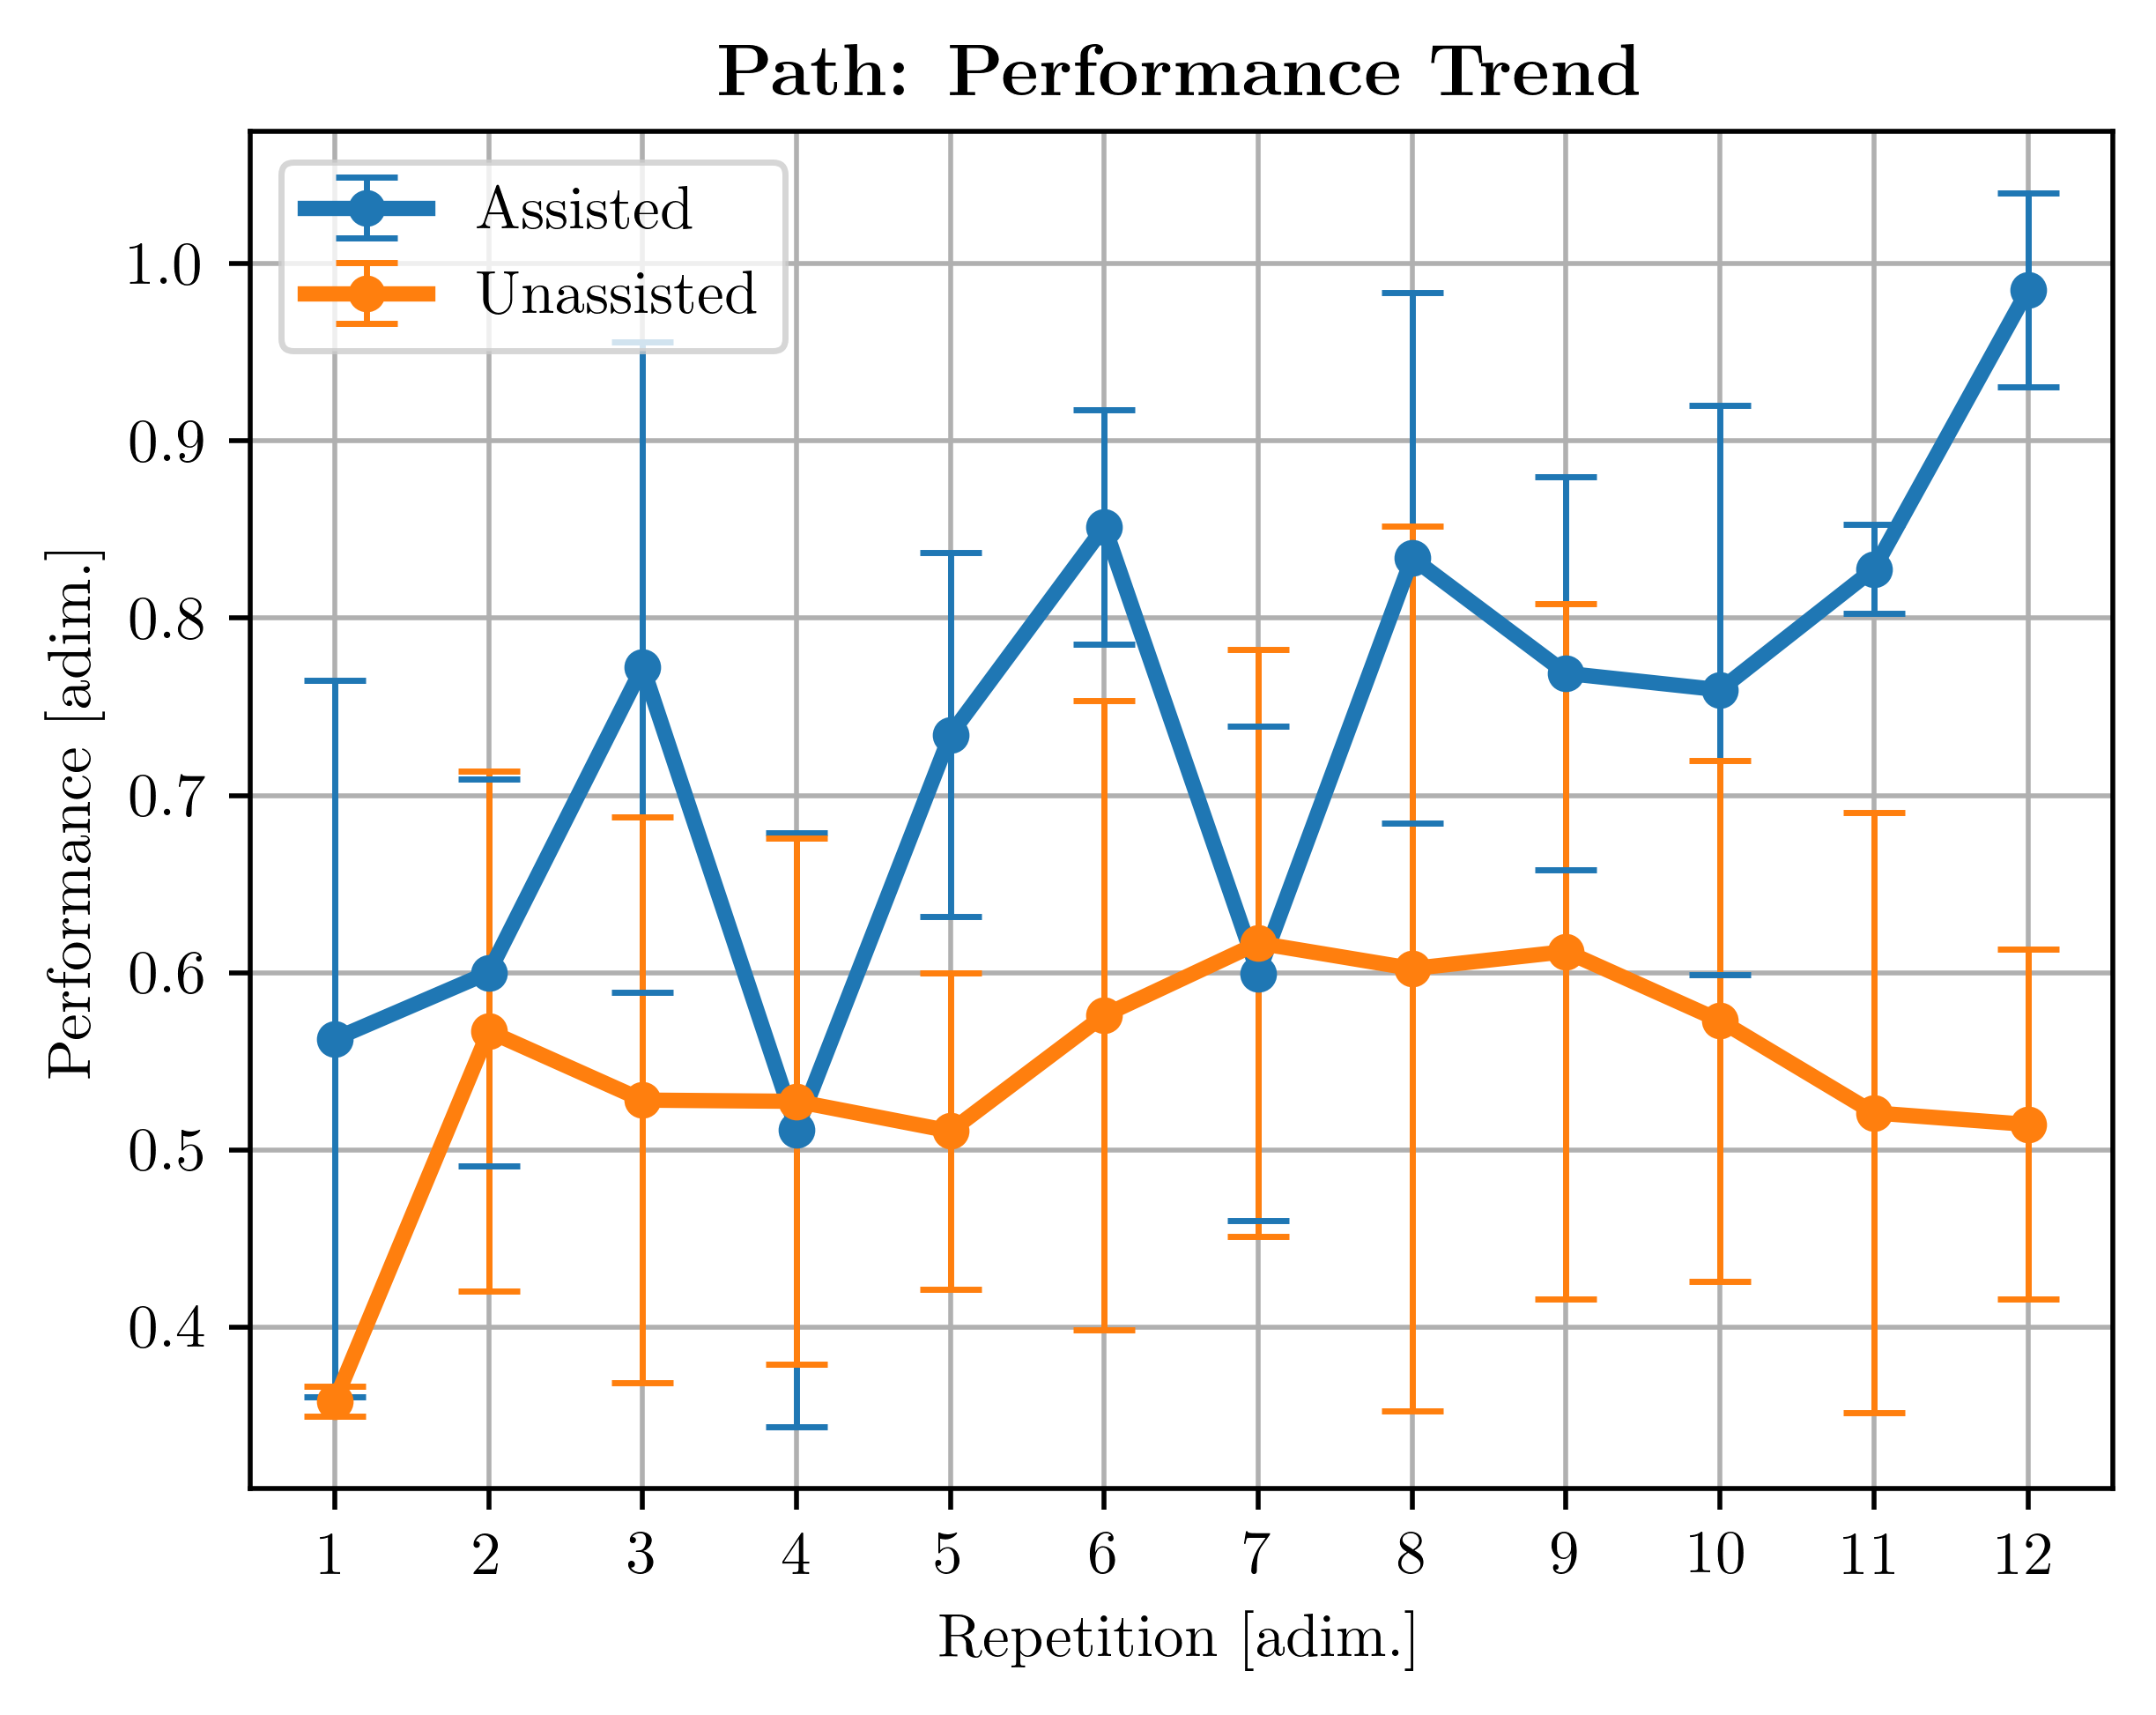
\includegraphics[width=\linewidth]{images/performance_training.png}
      \caption{\small{\textit{
        Performance Trend for the four Training Tasks. The value at each repetition is averaged across the subjects belonging to the same group. Error bars show the standard variation at each repetition
      }}}
      \label{fig:performancetraining}
\end{figure*}
\begin{figure*}
  \centering
      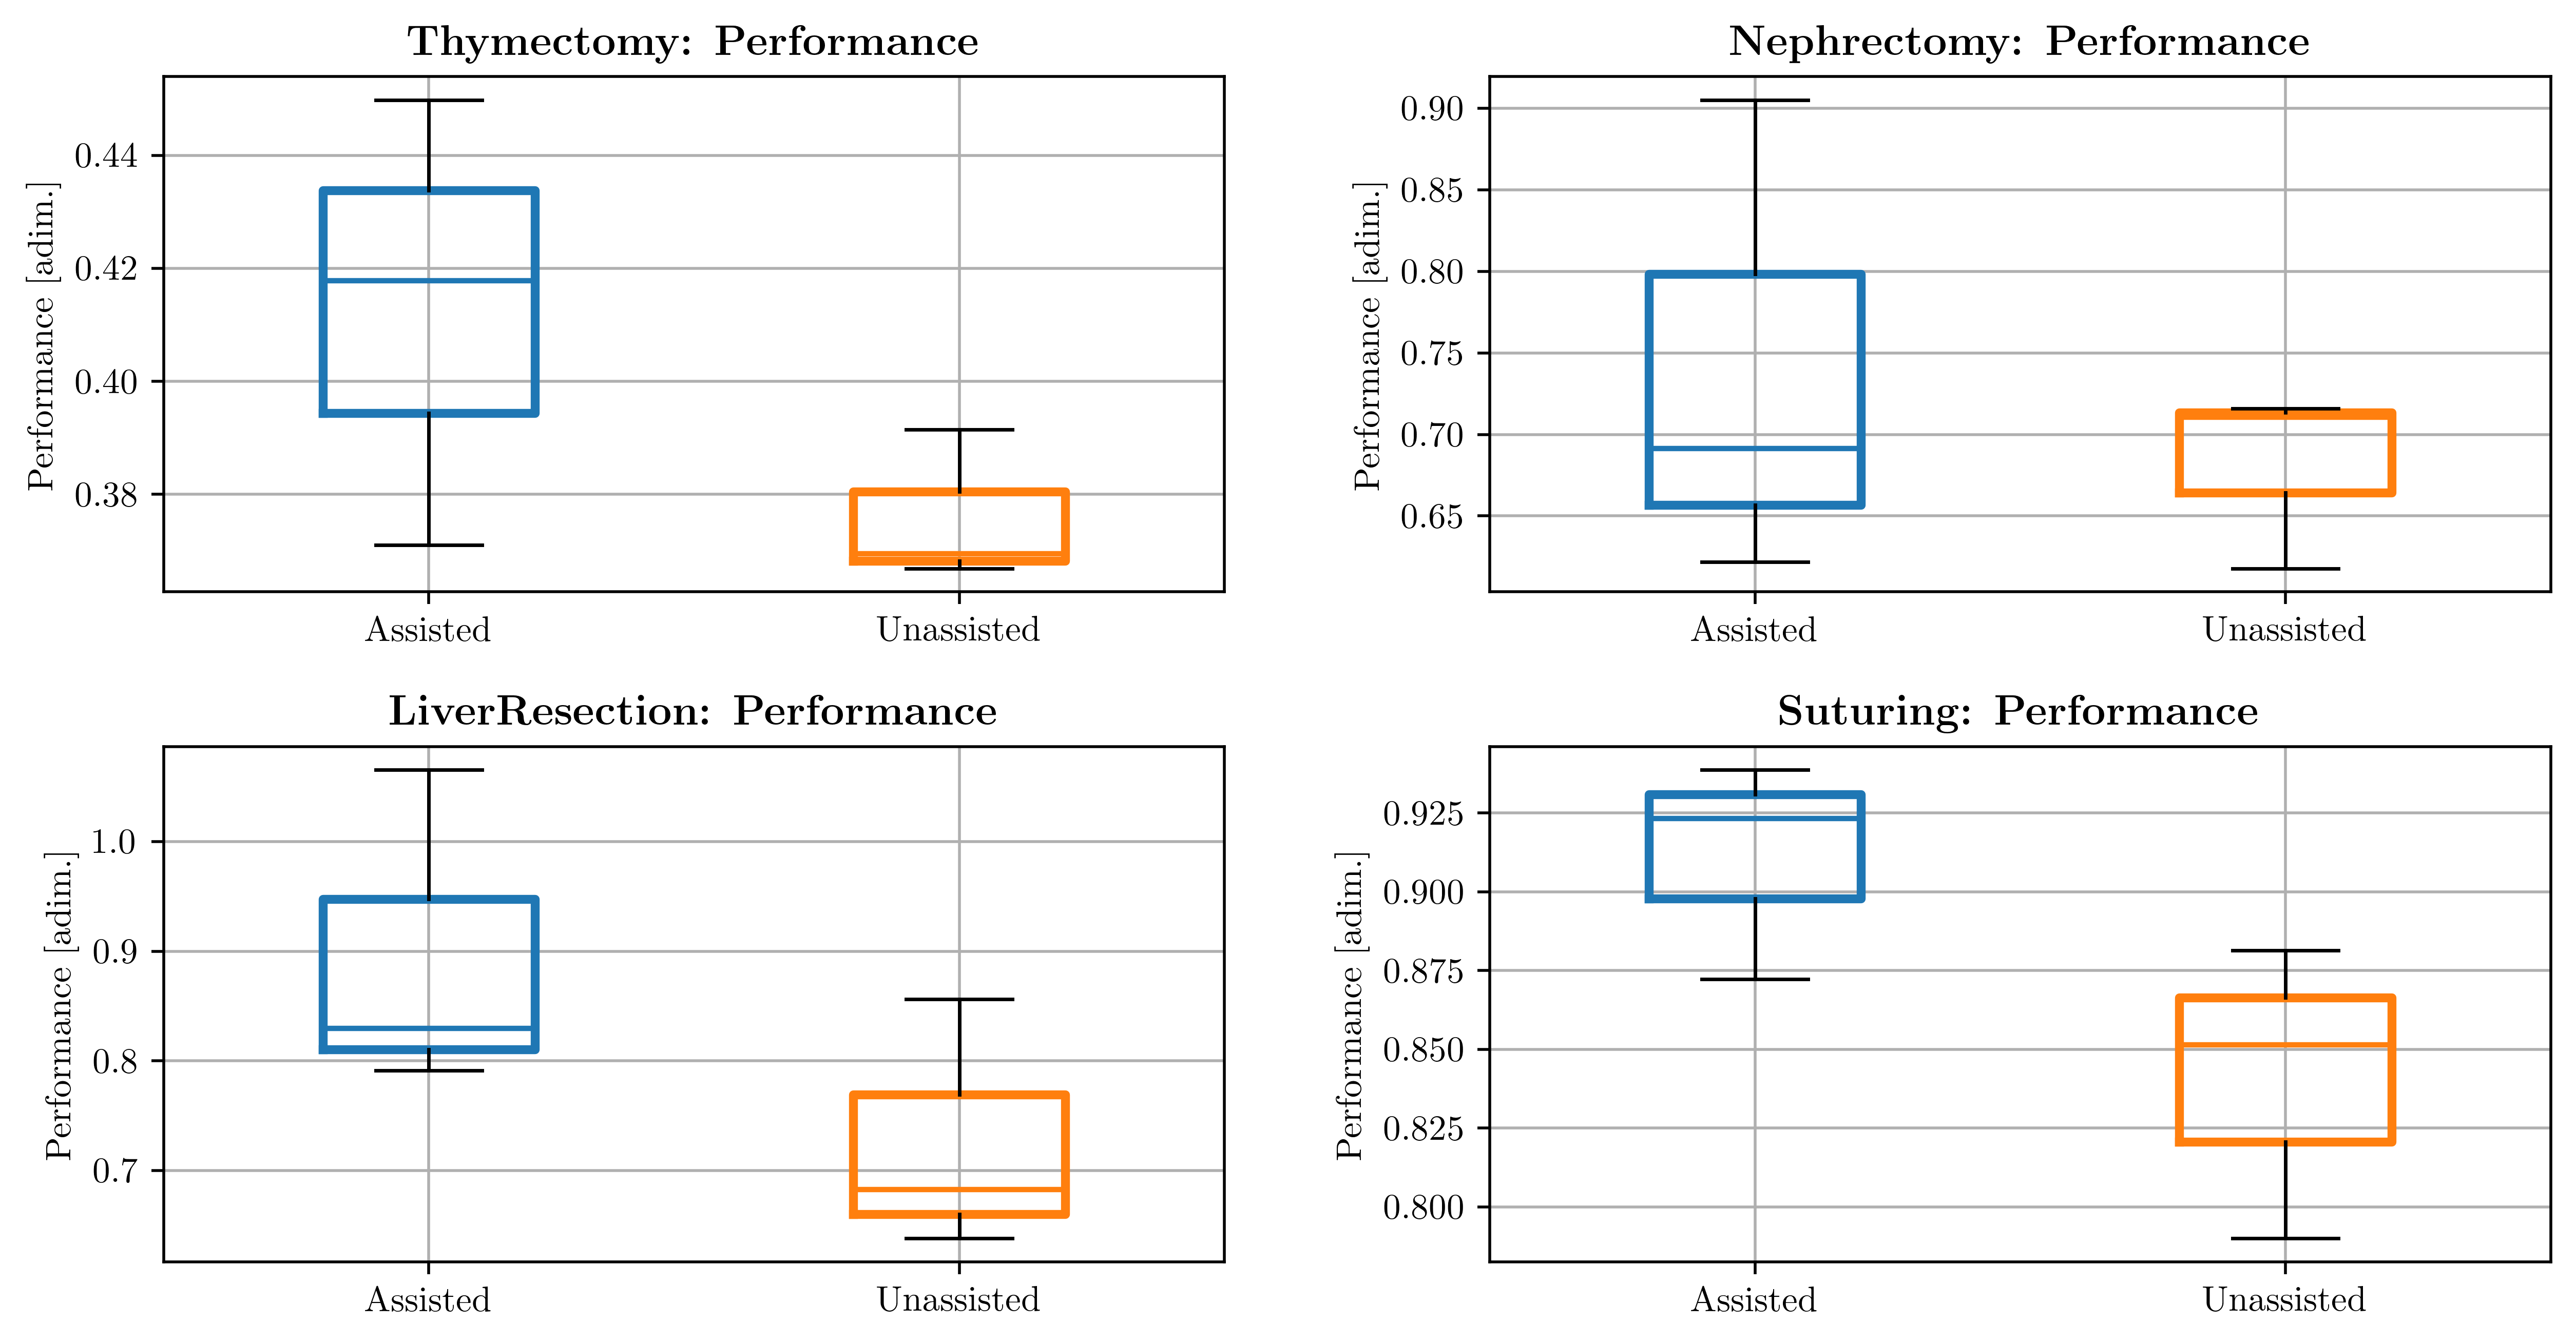
\includegraphics[width=\linewidth]{images/performance_validation.png}
      \caption{\small{\textit{
        Boxplots of the average performance of assisted subjects (blue) and unassisted subjects (orange) on the four validation tasks
      }}}
      \label{fig:performancevalidation}
\end{figure*}
Fig.\ref{fig:performancetraining} shows the performance trends for the four training tasks (\textit{Path, Rings, Pillars} and \textit{Exchange}), where the performance at each repetition is the average among the subjects in the assisted or control group. Apart from the \textit{Pillars} task, the trends are increasing both for the assisted group and the unassisted group. Most significantly, the performance in the assisted group is consistently higher than the one in the control group in all training tasks. 
\newline
The performance on the four validation tasks (\textit{Thymectomy, Nephrectomy, Liver Resection} and \textit{Suturing}) recorded on the last day of the experimental phase is shown in Fig.\ref{fig:performancevalidation} with boxplots. For each task, the graph reports the distribution of performances collected from the 4 subjects executing 3 repetitions. Crucially, neither the subjects in the assisted group nor the ones in the control group were guided with \acp{vf} on these tasks, nevertheless the performance recorded from the assisted subjects is distributed on higher values for all the tasks. 
\newline
Quantitative results are reported in the tables below: for each task, the mean, standard deviation and median values of performance are compared between the assisted and the control group. Given the data scarcity and their non-Gaussian distribution, the most meaningful conclusions will be drawn from the median values. Apart from \textit{Nephrectomy} showing a slightly reduced median performance on assisted subject (accompanied, however, by a much larger standard deviation, as per Fig.\ref{fig:performancevalidation}), all other tasks present an increase in both the mean and median performance, as high as $+21.54\%$.
\newline
The standard deviation in the performance isn't consistent when comparing the assisted and control group. 
\begin{center}
\begin{tabularx}{\linewidth}{||A|B|B|B||}
\hline
\multicolumn{4}{||c||}{\textbf{Thymectomy}} \\
\hline\hline
 & Mean & STD & Median \\
\hline
CONTROL & 0.38 & 0.01 & 0.37 \\
\hline
ASSISTED & 0.41 & 0.04 & 0.42 \\
\hline
\textbf{\% VAR} & \textbf{9.83\%} & \textbf{193.94\%} & \textbf{13.07\%} \\
\hline
% \label{tab:performance_Thymectomy}
\end{tabularx}
\end{center}
\begin{center}
\begin{tabularx}{\linewidth}{||A|B|B|B||}
\hline
\multicolumn{4}{||c||}{\textbf{Nephrectomy}} \\
\hline\hline
 & Mean & STD & Median \\
\hline
CONTROL & 0.68 & 0.06 & 0.71 \\
\hline
ASSISTED & 0.74 & 0.15 & 0.69 \\
\hline
\textbf{\% VAR} & \textbf{8.50\%} & \textbf{167.46\%} & \textbf{-2.71\%} \\
\hline
% \label{tab:performance_Nephrectomy}
\end{tabularx}
\end{center}
\begin{center}
\begin{tabularx}{\linewidth}{||A|B|B|B||}
\hline
\multicolumn{4}{||c||}{\textbf{LiverResection}} \\
\hline\hline
 & Mean & STD & Median \\
\hline
CONTROL & 0.73 & 0.12 & 0.68 \\
\hline
ASSISTED & 0.90 & 0.15 & 0.83 \\
\hline
\textbf{\% VAR} & \textbf{23.42\%} & \textbf{28.85\%} & \textbf{21.54\%} \\
\hline
% \label{tab:performance_LiverResection}
\end{tabularx}
\end{center}
\begin{center}
\begin{tabularx}{\linewidth}{||A|B|B|B||}
\hline
\multicolumn{4}{||c||}{\textbf{Suturing}} \\
\hline\hline
 & Mean & STD & Median \\
\hline
CONTROL & 0.84 & 0.05 & 0.85 \\
\hline
ASSISTED & 0.91 & 0.03 & 0.92 \\
\hline
\textbf{\% VAR} & \textbf{8.38\%} & \textbf{-25.39\%} & \textbf{8.44\%} \\
\hline
% \label{tab:performance_Suturing}
\end{tabularx}
\end{center}
\section{Discussion}
Graphs in Fig.\ref{fig:performancetraining} suggest that \acp{vf} grant a performance improvement when executing surgical tasks, an aspect that may be most beneficial in terms of safety and invasiveness when translated in the real surgical context. Under this light, haptic assistance effectively acts as an error-correction strategy which, when applied in real-time, re-directs the \ac{ee} towards safer spatial regions by acting on the master manipulators gripped by the surgeon.
\newline
Concerning the training experience and the associated learning curve, the available results do not show any significant difference when comparing the assisted and the control group, and the hypothesized benefits of \acp{vf} regarding this aspect remain to be verified.
\newline
The most interesting considerations may be drawn from Fig.\ref{fig:performancevalidation} where it's evident the difference in performance in favor of the assisted subjects. Since for these tasks, which were purposely designed to resemble real surgical scenarios, no haptic assistance was provided to either of the groups, it can be concluded that the introduction of haptic assistance in the training phase actively contributed to the skill transfer from training tasks to surgical tasks. This is arguably due to the integration of the haptic guidance into the visuo-haptic motor feedback loop that acts during teleoperation: \acp{vf} therefore contribute to motor learning and, ultimately, improve the establishment of surgical skills in the longer run. As a consequence, the benefits of employing haptic assistance could arise after the training phase as well, when Virtual Fixtures are not in use.
\section{Conclusions}
This work features the development of a haptic-enhanced VR surgical simulator integrated with a \textit{daVinci}\cright robot and an experimental study on the role of Virtual Fixtures employed as assistance strategies in the surgical training context. The results of the experimental study have concluded that employing \acp{vf} during the training phase of surgical practice leads to improved performance and augmented skill transfer toward real surgical scenarios where haptic assistance is absent.

%-----------------------------------------------------------------------------------
% BIBLIOGRAPHY
\bibliographystyle{unsrt}
\bibliography{refs.bib}
%-----------------------------------------------------------------------------------
\end{multicols}
\end{document}


